\chapter{Research Methodology and Data}

This chapter focuses on describing which approaches were chosen for the task at hand and why, as well as shows how the work progressed. 

\section{Core Concepts}

To reiterate the current problem is to find out if \gls{gnn} can compete at solving the \gls{mwm} problem compared to other options such as greedy algorithm.

Before properly describing the choices made for approaching this problem, it is worth going through basic concepts of \gls{gnn}s and neural networks in general. It is common to think of neural networks as of a black box where you give some data to this box and it gives back an answer. In this case the data is a graph consisting of vertices connected by edges that have weights and the expected answer should be pairs of vertices that were matched together. This is however not as straight forward as the more common examples of classification where each data item needs to be classified.  


Supervised learning has one side effect

\section{Challenges}

As mentioned the idea behind supervised learning is to give a model the correct answers so it can by trial and error learn from it. Theese answers are not included the initial datasets so the optimal solutions need to be calculated. Blossom algorithm implemented by Joris van Rantwijk in Python was used \cite{mwmBlossom}. This does however point out an important weakness of the supervised approach. Obviously a model needs to be able to handle graphs of different sizes and it is the large ones that are most interesting. Finding an optimal \gls{mwm} for the large graphs can be time consuming, at the same time a model need as much data as possible to learn leading to multiple large graphs consuming to much time. This poses a question whether it is possible for the model to learn on small and medium sized graphs that are not as time consuming and transfer learned patterns to solve larger graphs.


\section{Data}

The model should be capable of solving any graph relevant to \gls{mwm} problem. A relevant graph can be difined by following characterisitcs
Ideally the model should be able to handle any kind of a graph with weighted edges.


\section{Expected Results}

\subsection{Accuracy and total weight}

There are not that many researches specifically for \gls{mwm}, but problems like \gls{mis} that are relatively close to \gls{mwm} can indicate similar results for this case as well. As discussed in the \hyperref[sec:background]{Background section}, there are researches that show that \gls{gnn}s are capable of solving \gls{co} problems and beating greedy algorithms, while other rather indicate that improvements are still needed for it to be worth using. Therefore it is hard to forecast any results based on previous work. Nothing stands in the way of being optimistic however, additionally to the fact that greedy algorithm is relatively simple and \gls{nn} should be able the recognise a more complex pattern it can use to achieve better results. It is absolutely not expected for the model to be able to find optimal solution since any \gls{nn} is a heuristic. The margin by which \gls{gnn} can surpass the greedy solution is expected to be rather small, since from the data analysis it was abserved that for the majority of graphs greedy algorithm preforms rather well with above 80\% of the optimal possible weight.

\subsection{Time}

\gls{gnn} model is a heuristic solver and gives an approximate answer. Therefore model should be noticeably faster than exact algorithm, otherwise it would not be worth it. The time a model takes to solve one instance of a problem should be closer to that of a greedy algorithm and probably slightly longer due to preproccessing required such as augmenting data with adittional features. Naturaly, time will also depend on the depth and the width of the network.

\section{Model Architecture}



\section{Line Graph Approach}

Line graph approach was the first attempt at using a simple \gls{gnn}, which later turned out to be too time consuming for larger graphs to be worth further expriements. It did however give some usefull insight as well as a showed to be a proof of concept. In the context of graphs line graph is a complement of the original graph that turns each edge to a vertex and connects the vertices is they shared a vertex in the original graph. 

Nouranizadeh et. al. showed anothing approach at solving \gls{mis} \cite{DBLPjournals/corr/abs-2107-01410}.

Examaple of a graph and its line graph convertion
\begin{figure}[H]
    \centering
    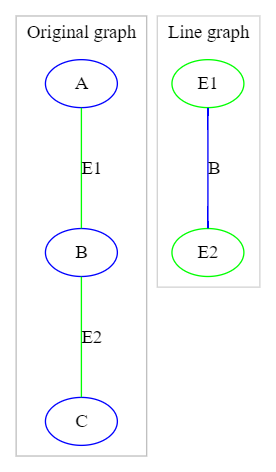
\includegraphics[scale=0.5]{figures/LineGraphExample}
    \caption{Original graph (left) and its line graph (right)}
    \label{Line graph figure}
\end{figure}

\subsection{Progress}

1. bare bones
2. class weights -> all or nothing
3. optimizer learning rate, network depth and width, 
4. skip connections
5. extra features


\section{Edge Classification Approach}

A more natural way of approaching this problem is for each pair of vertices that are conneced by an edge, ask the model if given pair should be a part of the matching. In other words model is classifying an edge. 

\subsection{Progress}

\section{Result Validation}

\begin{enumerate}
\item Time - how long an algorithm took to produce an answer.
\item Correctness - is the answer correct. In case of \gls{mwm} the total weight aquired would be the measurement of how correct the solution is. It is unlikely that \gls{gnn} can find an optimal solution for more complex problems so it is reasonable to look at how close \gls{gnn} comes to the optimal solution.
\item Memory - how much memory is needed. However in this project there is less of a focus on memory
\end{enumerate}

All the experiments have been done on the same machine with: 11th Gen Intel(R) Core(TM) i7-11700K 3.60GHz 8-core CPU, 16 GB RAM and NVIDIA RTX 3080Ti graphics card.


